\label{sec:other_model}

My personal contribution to this chapter \cite{carpentier:hal-01203507} is on the experimentation on the real robot.
I will therefore briefly depict the general idea corresponding to the OCP and present in a bit more detail the performance and the experiments done with this formulation.

\subsection*{OCP formulation}

As explained in the paragraph named \emph{Formulation} in \cite{carpentier:hal-01203507}, the OCP is as follow :

\begin{subequations} \label{eq:ocp}
\begin{eqnarray}
\hspace{-3em}	\underset{\substack{\hspace{2.2em} \underline{\bm x}=(\bm c, \bm h, \am), \\ \underline{\bm u}=\bm\phi} }{\min } \ \ \  
	& & \hspace{-3.5em} \int_{0}^{T} \ell_h(\bm x) + \ell_\kappa(\bm x) + \ell_\am(\dot{\bm x}) + \ell_\phi(\bm u) \, dt \label{eq:cost2} \\
	s.t. & \forall t & \dot{\bm{x}} = f(\bm x, \bm u) \label{eq:dyn_constraint2} \\
	&  \forall t& \bm\phi \in \mathcal{K} 	\label{eq:conic_constraint2} \\
	& & \bm x(0) = (\bm c_{0},\bm 0,\bm 0)  \label{eq:init_constraint2} \\
	& & \bm x(T) = (\bm c^*,\bm 0,\bm 0)  \label{eq:term_constraint2} \\
        & &  \dot{\bm h}(0) = \dot \am(0) = \dot{\bm h}(T) =\dot\am(T) = \bm 0  \label{eq:add_constraint2}
\end{eqnarray}
\end{subequations}
where:
\begin{list}{ \arabic{point}.}{%
		\usecounter{point}%
		\setlength{\topsep}{5pt}%
		\setlength{\itemsep}{0pt}%
		\setlength{\parsep}{0pt}%
		\setlength{\labelwidth}{3.em}%
		\setlength{\leftmargin}{2em}%
		\setlength{\labelsep}{0.5em}%
	}
\item[*] $\ell_h(x) = \lambda_h || \bm  h ||^2$ is the norm of the linear momentum,
\item[*] $\ell_\kappa(\bm x) = \sum_{k=1}^K \kappa(\bm c, \bm p_k)$ represents the kinematic limits of the robot's whole body by setting an exponential barrier on the distance between the COM and the contact points:
\begin{equation}
	\kappa (\bm c, \bm p_{k}) = 
	\exp(\|\bm c - \bm p_{k}\| - u_{b})
	+
	\exp(-\|\bm c - \bm p_{k}\| + l_{b})
\end{equation}
\item[*] $\ell_\am(\dot{\bm x}) = \lambda_\am || \dot \am ||^2$ is the norm of the angular momentum time derivative,
\item[*] $\ell_\phi(\bm u) = || \bm\phi ||^2$ is the norm of the forces applied at the contact point,
\item[*] $ \dot{\bm{x}} = f(\bm x, \bm u) $ is the equation of the template model dynamics,
\item[*] $u_{b}$, $l_{b}$ are the arbitrary upper and lower bounds,
\item[*] the weight $\lambda_h$ is adapted depending on the phase: for support phase involving large displacement (like a large movement of the swing foot), the weight is divided by 10 with respect to its nominal value,
\item[*] and $\mathcal{K}$ are the friction cones.
\end{list}

The main differences between both formulations are:
\begin{list}{ \arabic{point}.}{%
		\usecounter{point}%
		\setlength{\topsep}{5pt}%
		\setlength{\itemsep}{0pt}%
		\setlength{\parsep}{0pt}%
		\setlength{\labelwidth}{3.em}%
		\setlength{\leftmargin}{2em}%
		\setlength{\labelsep}{0.5em}%
	}
\item[-] the shape of the cost function,
\item[-] how the problem is regulated via a slack variable Eq.~\eqref{eq:optimal_control_problem} or not Eq.~\eqref{eq:ocp},
\item[-] the parametrization of the system,
\item[-] the use of sparsity,
\item[-] and how linear constraint are represented in the problem.
\end{list} 
It appeared that the second formulation is much more appropriate for the solver. 

\subsection*{Experimental results}

\begin{figure*}[!ht]
  \begin{center}
  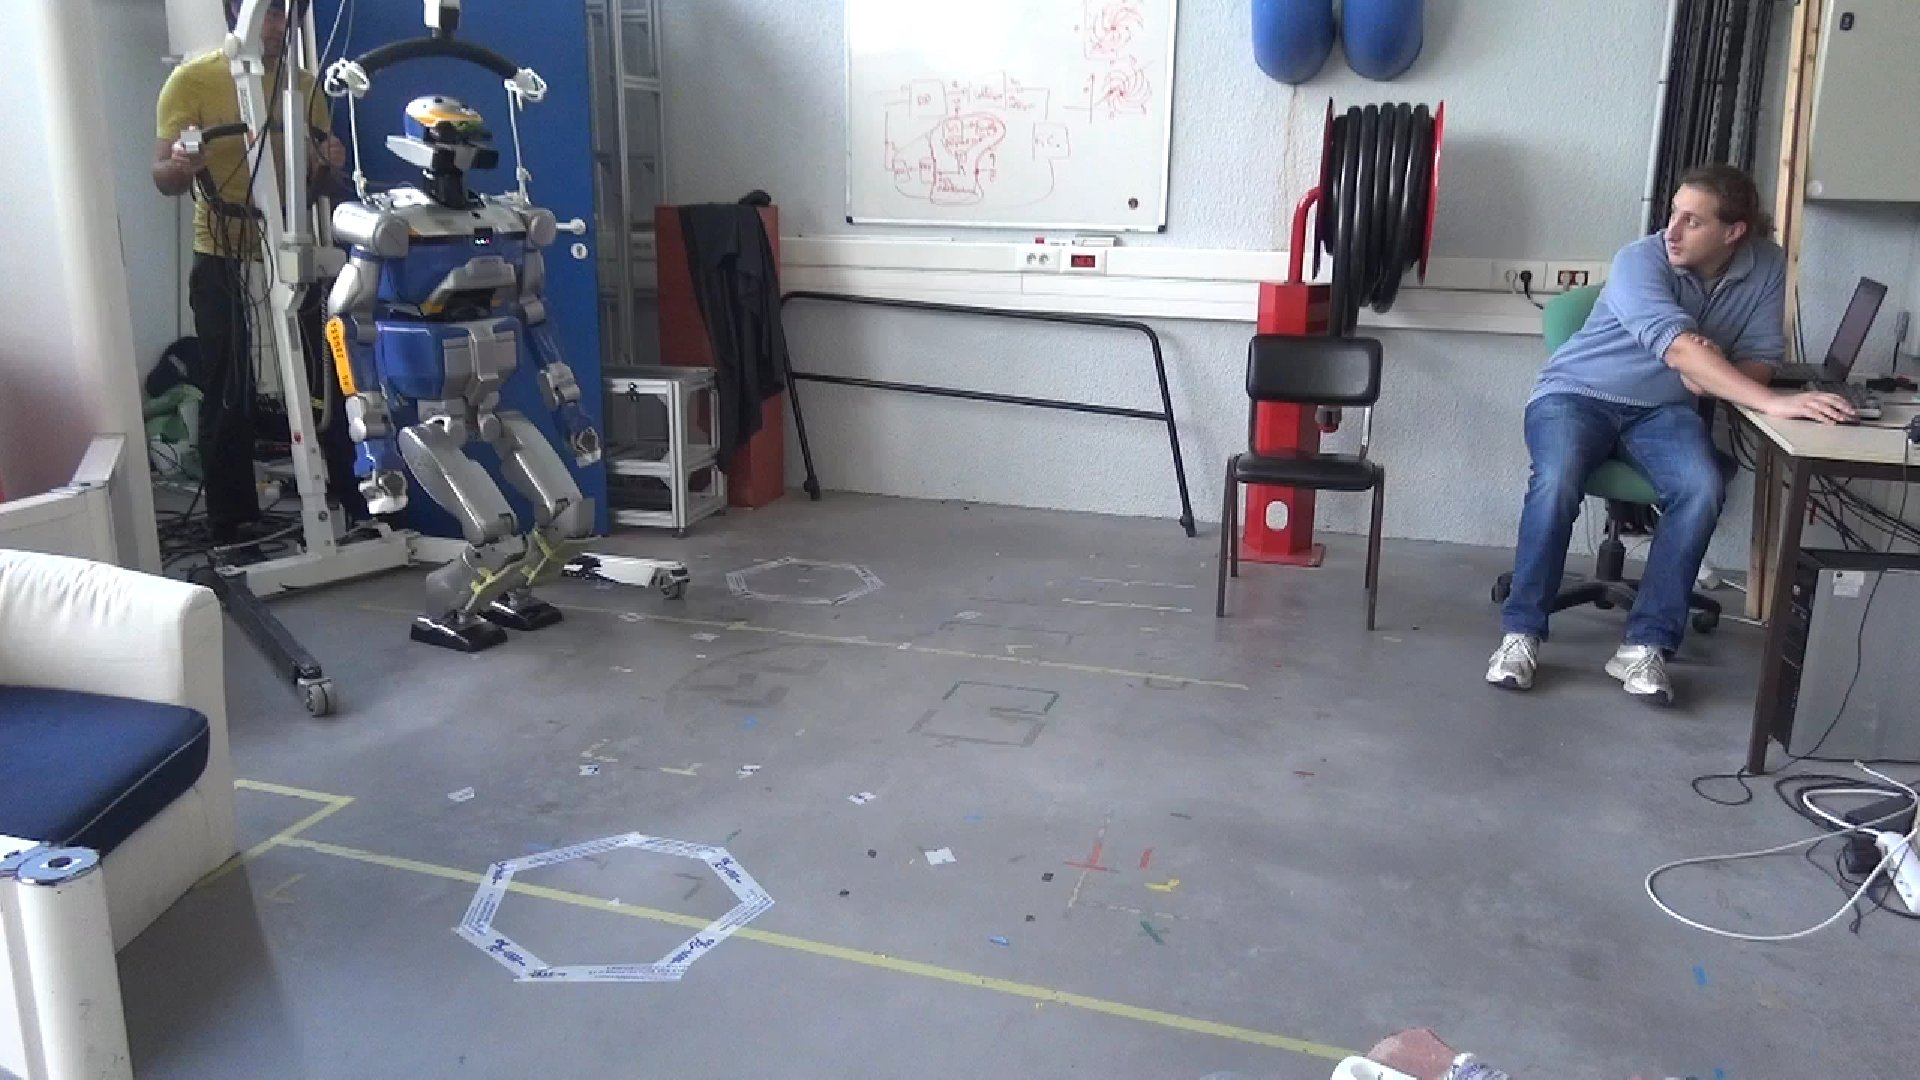
\includegraphics[trim={7.0cm 0.0cm 20.0cm 0.0cm}, clip, width=0.18\linewidth]
    {./Multicontact/MulticontactJustin/fig/fastwalk1.jpeg}
  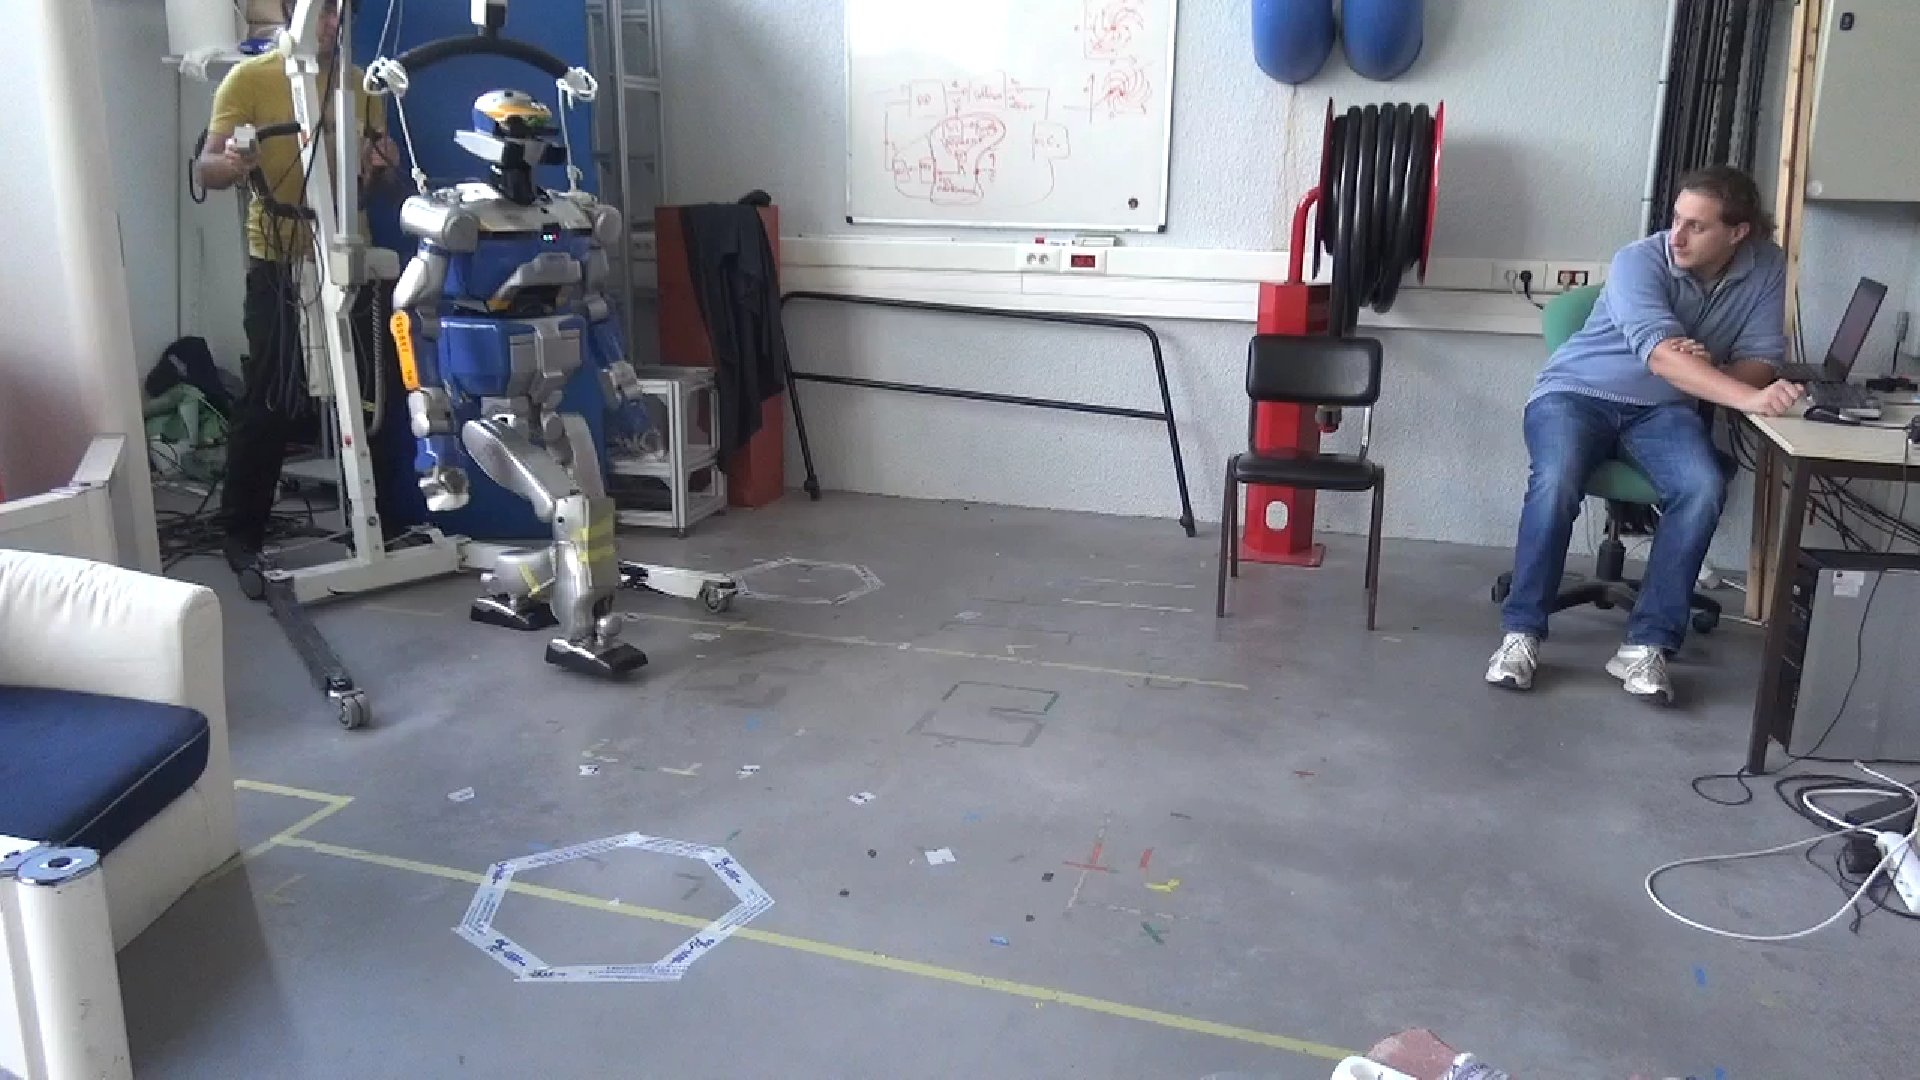
\includegraphics[trim={7.0cm 0.0cm 20.0cm 0.0cm}, clip, width=0.18\linewidth]
    {./Multicontact/MulticontactJustin/fig/fastwalk2.jpeg}
  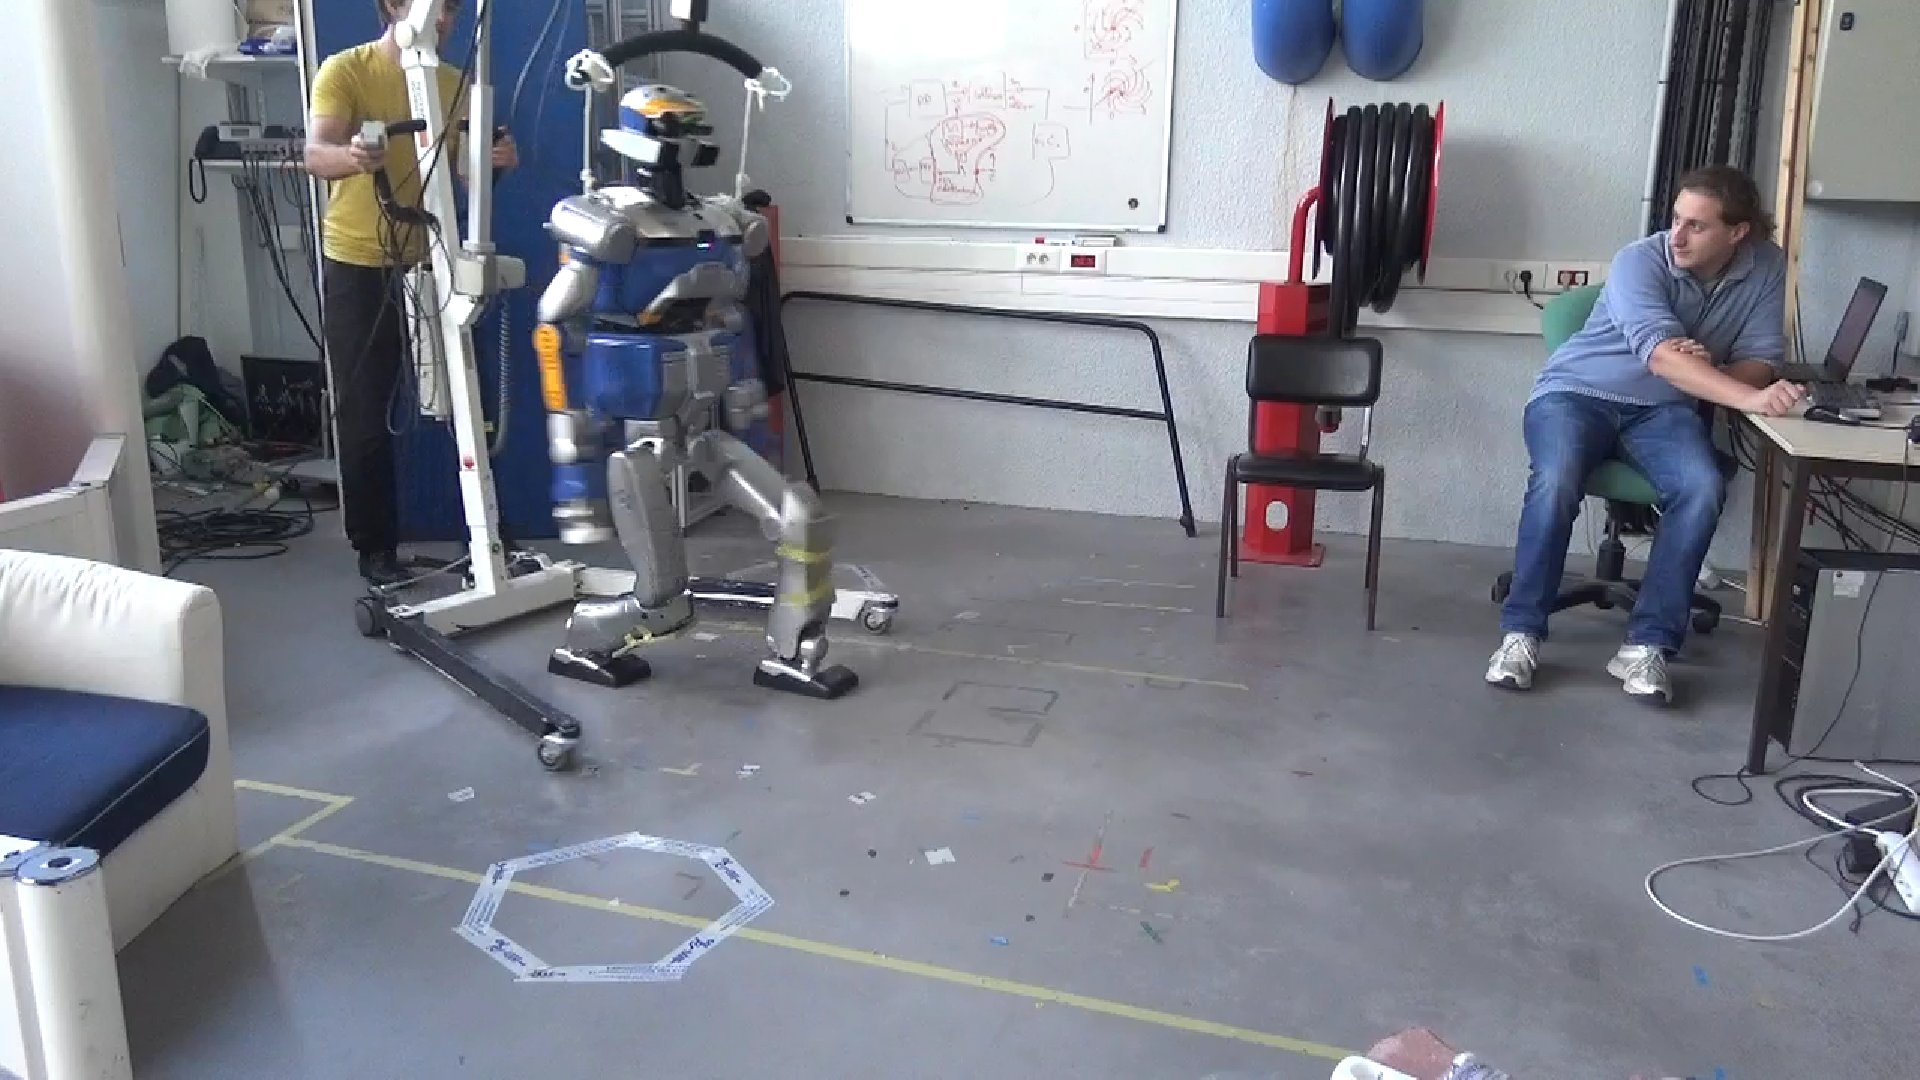
\includegraphics[trim={7.0cm 0.0cm 20.0cm 0.0cm}, clip, width=0.18\linewidth]
    {./Multicontact/MulticontactJustin/fig/fastwalk3.jpeg}
  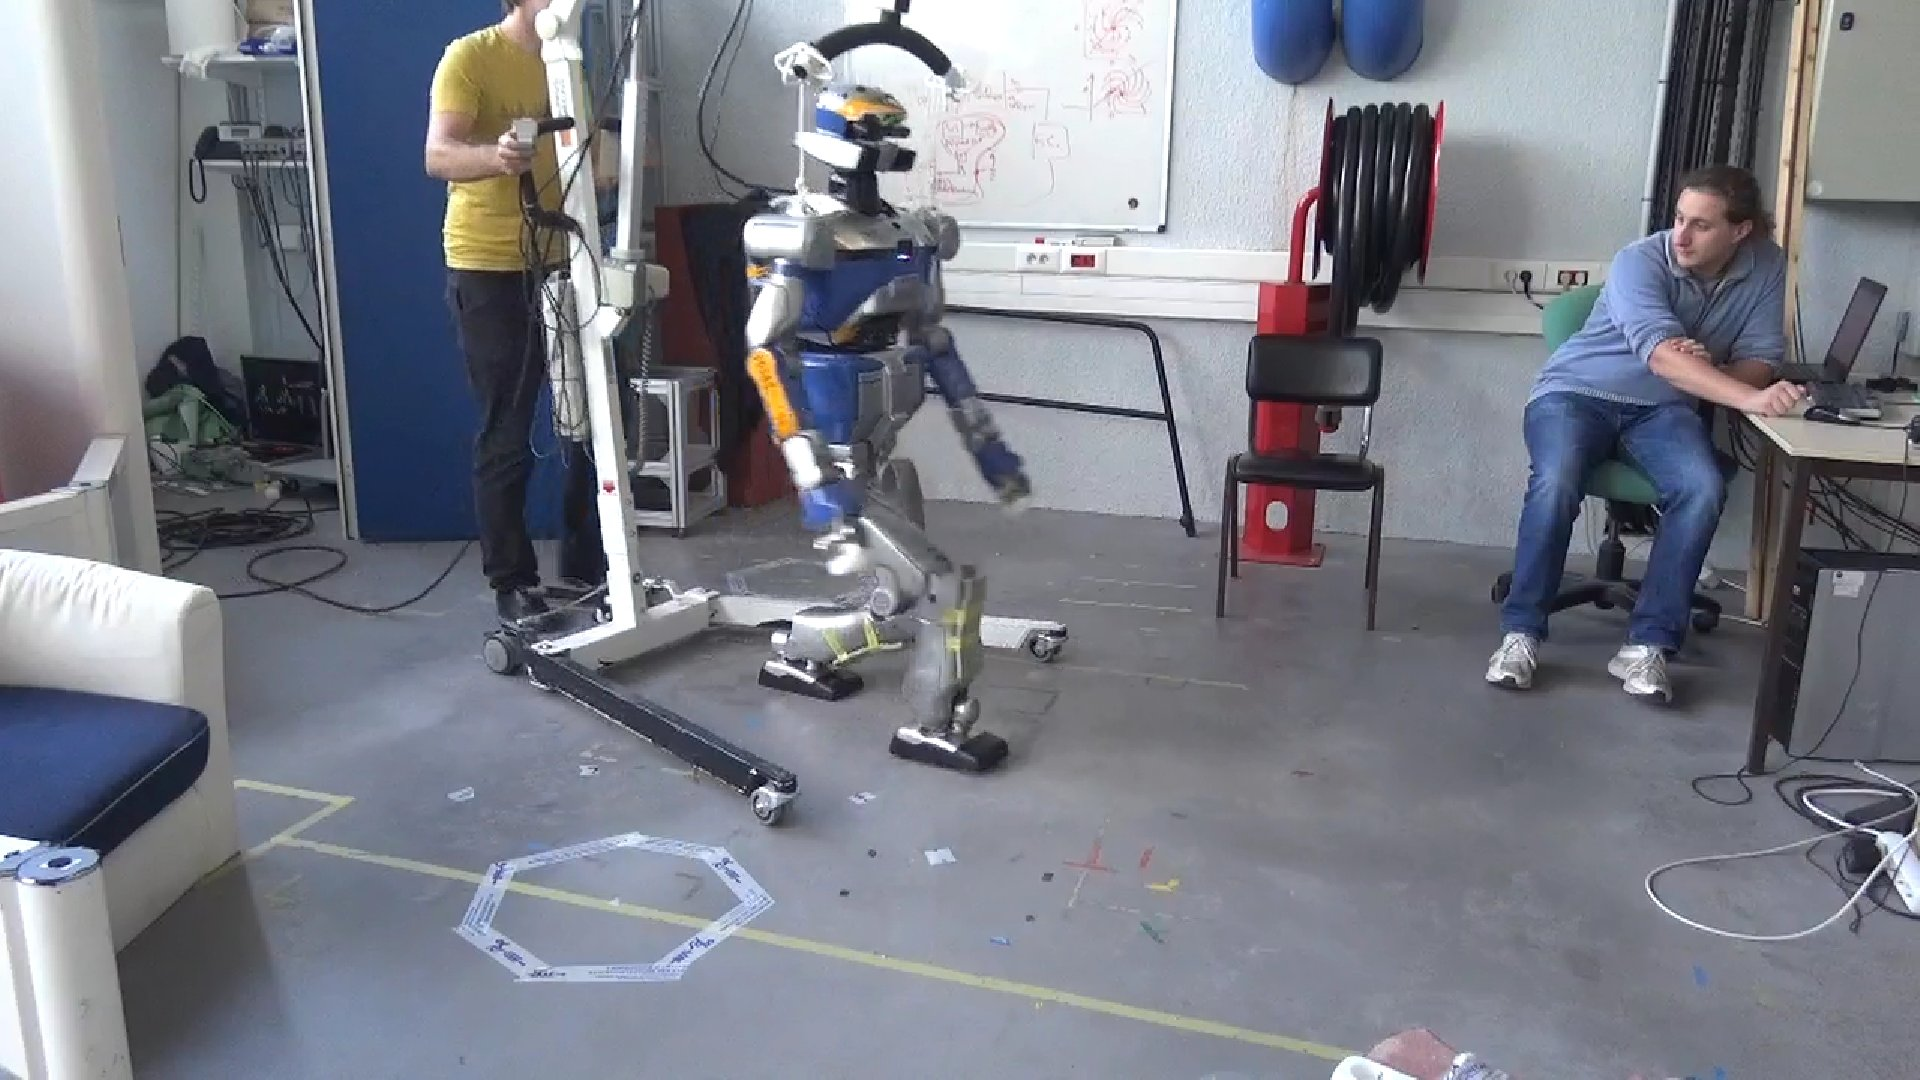
\includegraphics[trim={7.0cm 0.0cm 20.0cm 0.0cm}, clip, width=0.18\linewidth]
    {./Multicontact/MulticontactJustin/fig/fastwalk4.jpeg}
  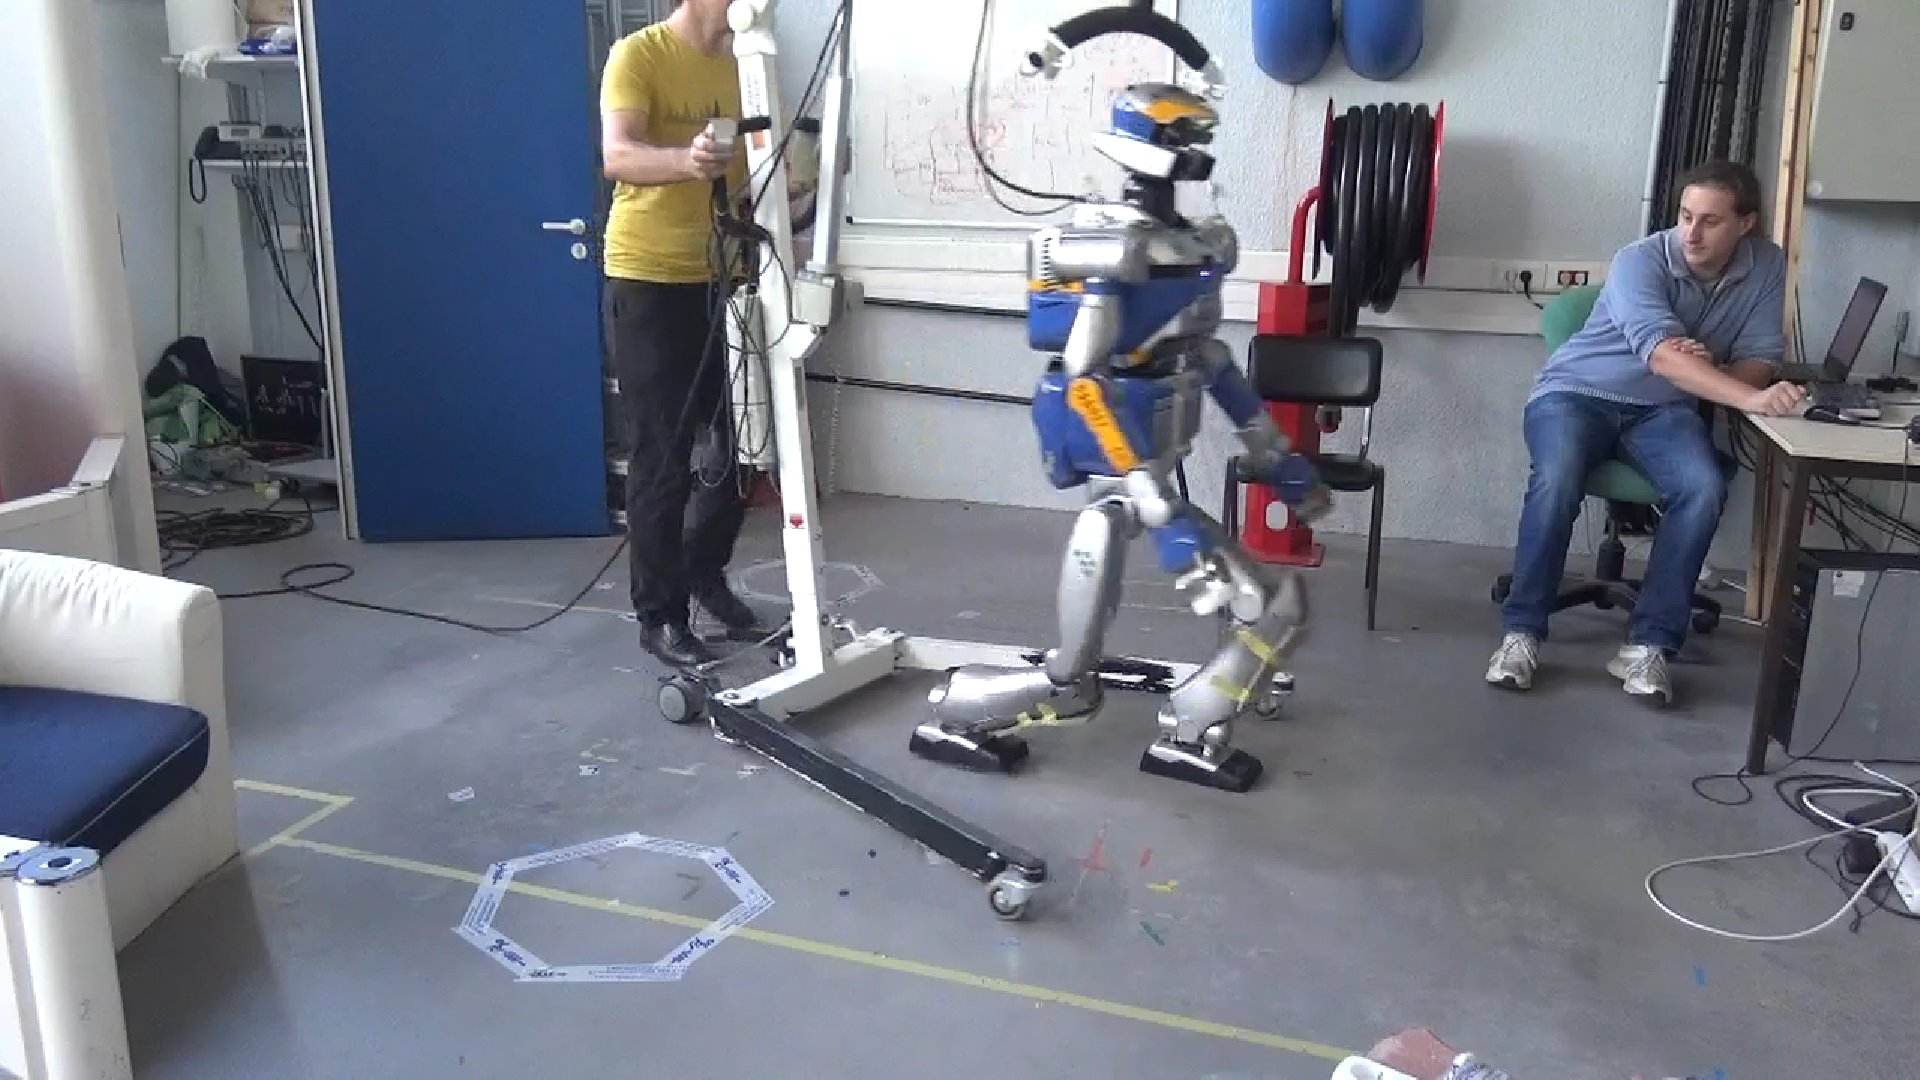
\includegraphics[trim={18.0cm 0.0cm 10.0cm 0.0cm}, clip, width=0.18\linewidth]
    {./Multicontact/MulticontactJustin/fig/fastwalk5.jpeg}
  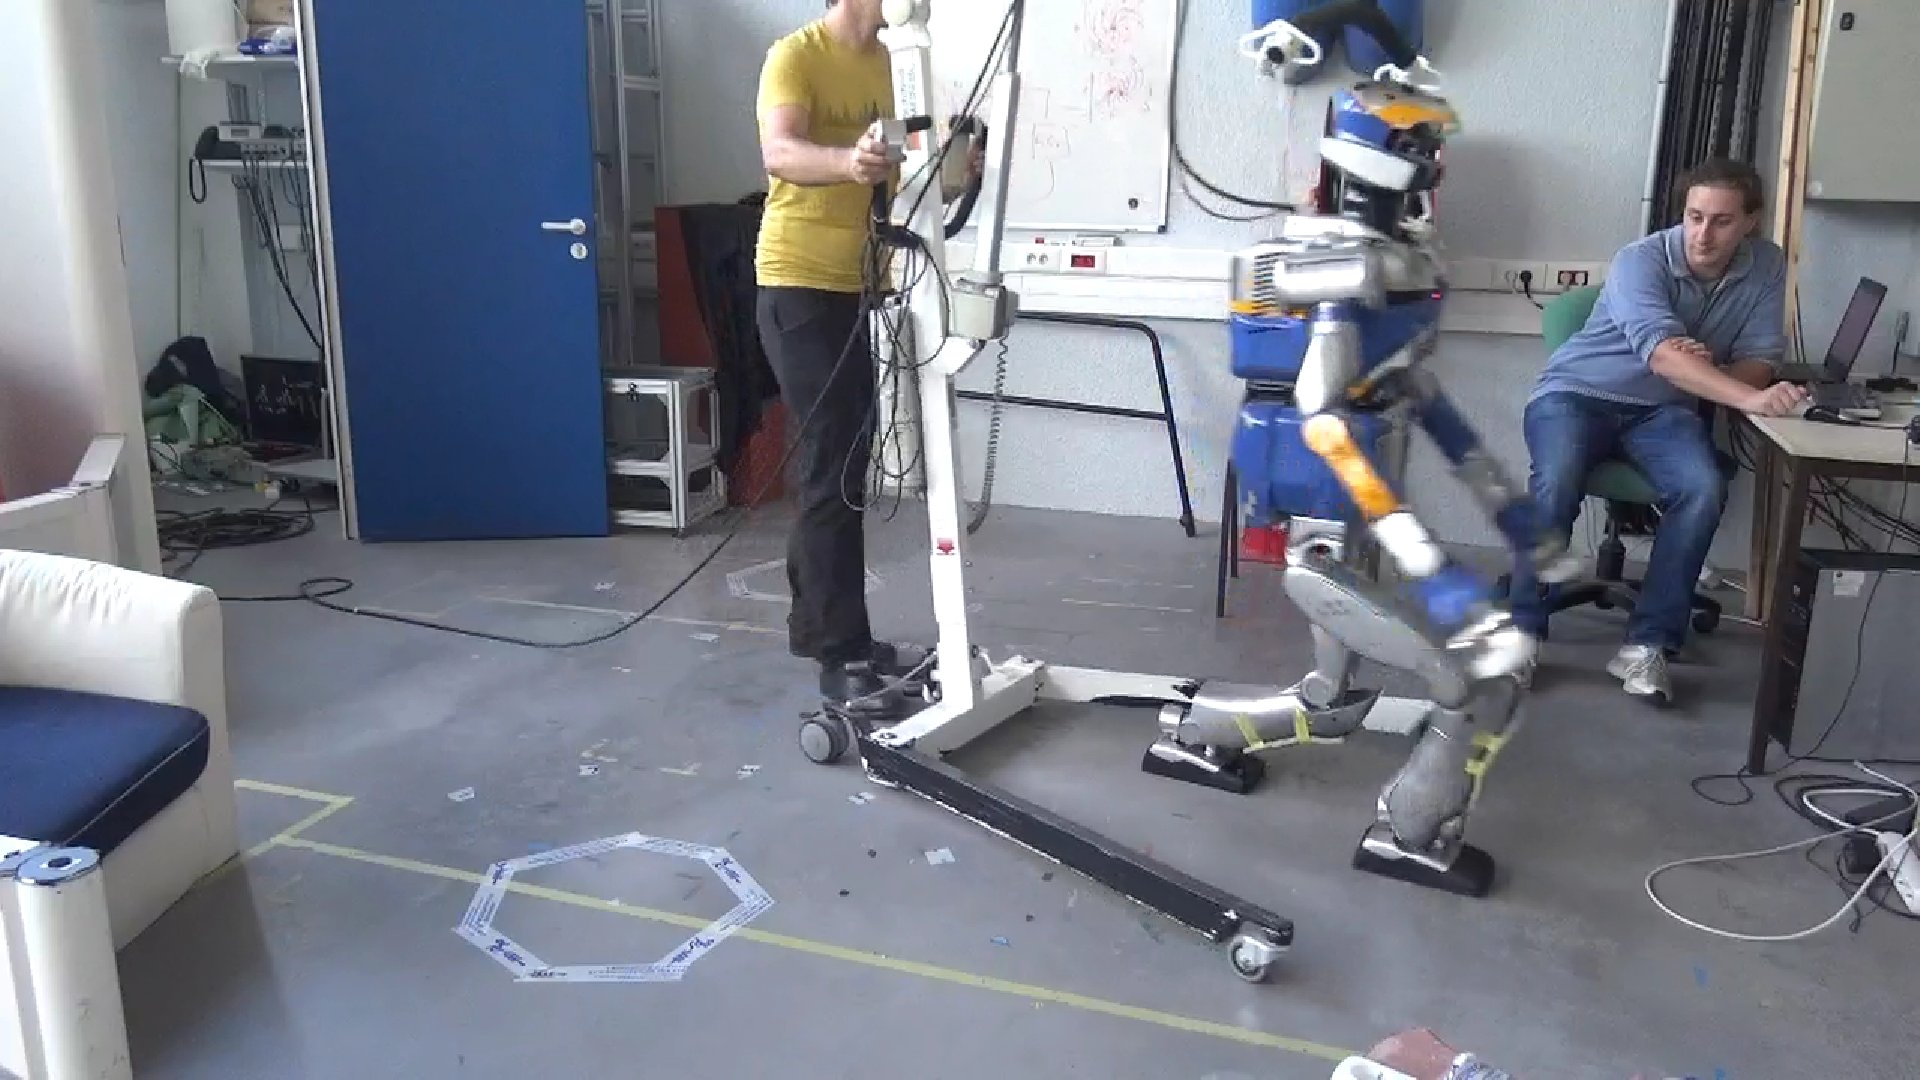
\includegraphics[trim={23.0cm 0.0cm 5.0cm 0.0cm}, clip, width=0.18\linewidth]
    {./Multicontact/MulticontactJustin/fig/fastwalk6.jpeg}
  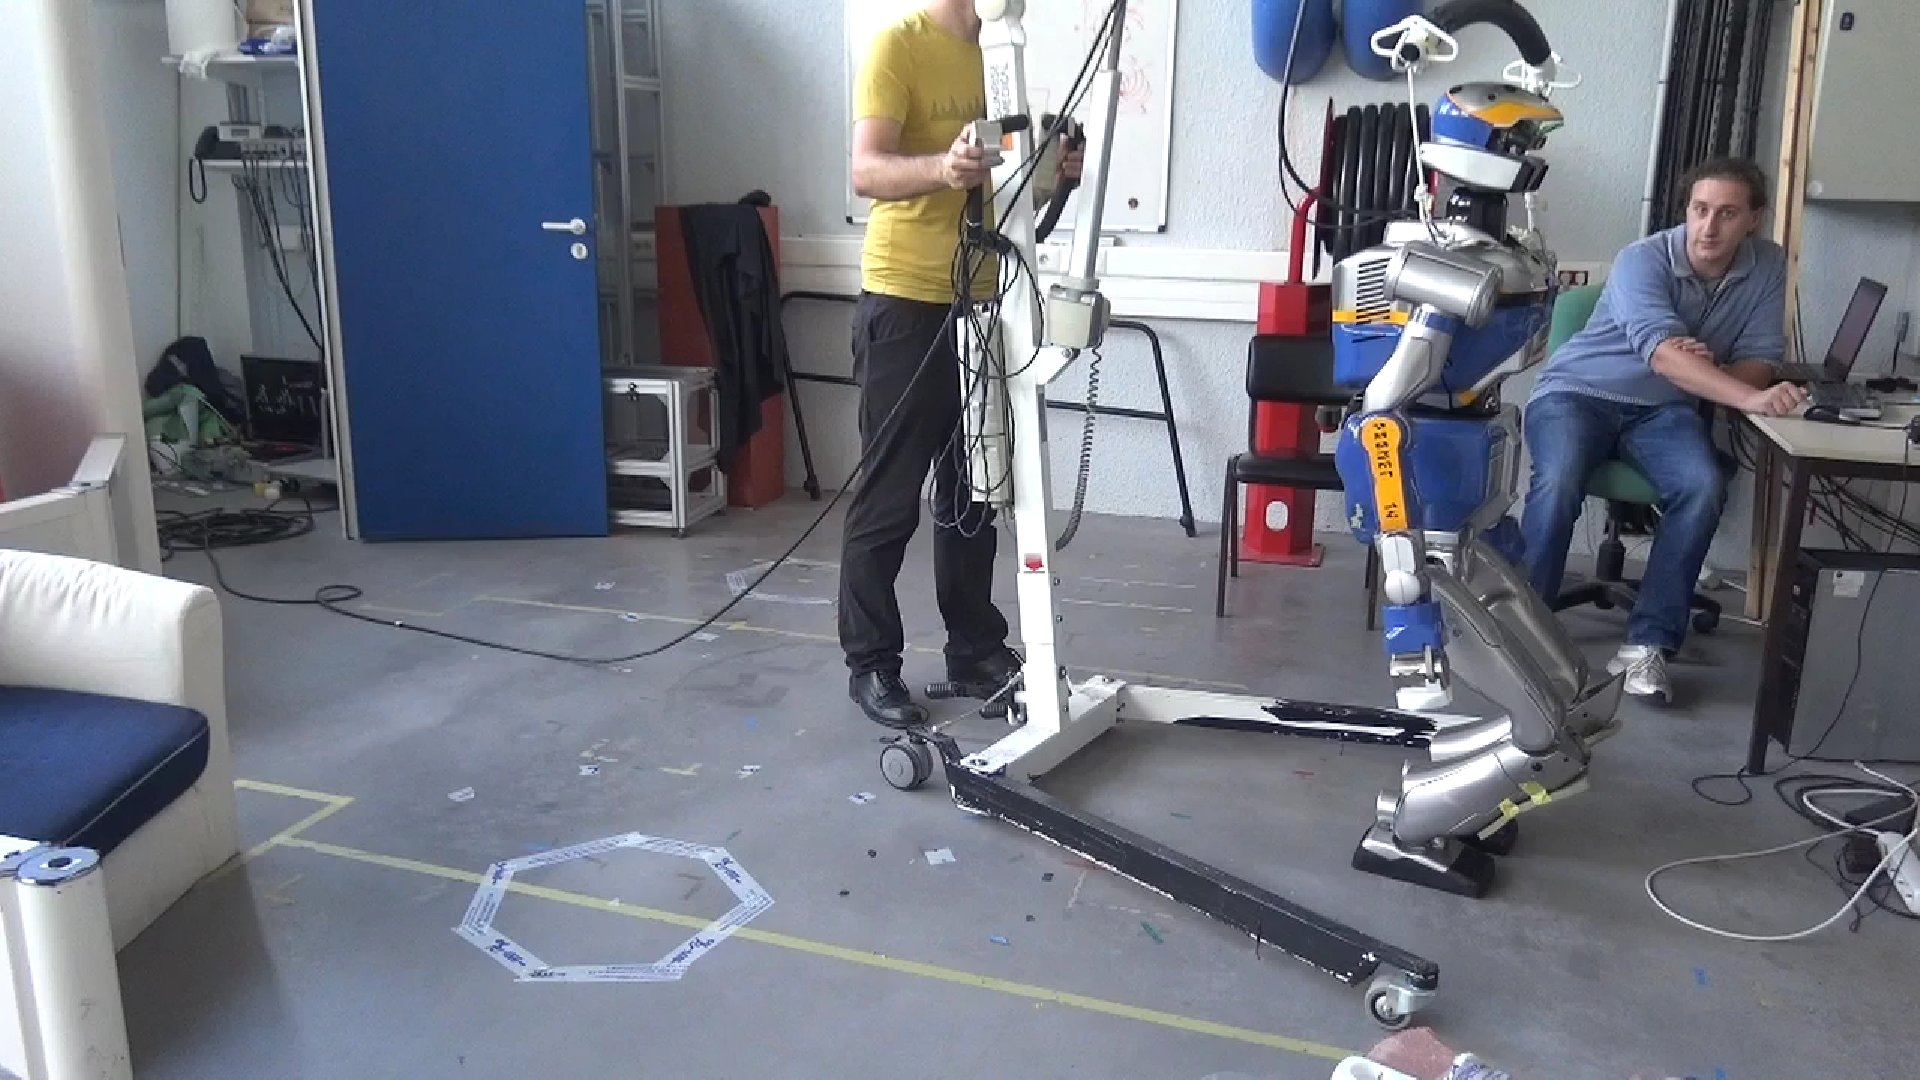
\includegraphics[trim={23.0cm 0.0cm 5.0cm 0.0cm}, clip, width=0.18\linewidth]
    {./Multicontact/MulticontactJustin/fig/fastwalk7.jpeg}
  \caption{
    Experiment 1: Walking in straight line with enjambment of $100cm$.
  }
  \label{fig:moviepicture}
  \end{center}
\end{figure*}

Two main experiments carried out on the HRP-2 robot are presented. The first experiment concerns the generation of a classic walking motion: it is a unitary test but it is important to properly understand the behavior of our solver compared to classical walking pattern generators. The second experiment is the same climbing stairs scenario depicted in Fig. \ref{fig:moviepicture} and in Fig. \ref{fig:contact_stances}, where the robot has to make use of the handrail to help its ascension of the stairs. 
Additional movements of running and standing up were simulated but not executed by the robot so the user is kindly asked to look at \cite{carpentier:hal-01203507} for more details.

\subsection*{Experimental setup}

All the computations (contact planning and WPG) were performed offline on a Intel Xeon(R) CPU E3-1240 v3 @ 3.40GHz.
In this case the contact planner used is the open-source Humanoid Path Planner available at \url{https://github.com/humanoid-path-planner}.
The OCP is also solved using the proprietary software MUSCOD provided by the Interdisciplinary Center for Scientific Computing (IWR) of Heidelberg University.
In this experiment, however, we used the sparsity solver to solve the problem.
For the walking experiments, we used a closed-loop control provided with the robot (called the stabilizer) to stabilize the movements of the rubber bush inside each foot~\cite{6942670}.
The stabilizer was not used for climbing the stairs, because it is not able to handle hand contacts.

\subsubsection*{Experiment 1: large enjambment on a flat ground}

In this first experiment, a sequence of cyclic contacts is manually generated with enjambment of $100\,cm$.
The timings are fixed (single support: $1.0\,s$; double support: $0.1\,s$). The total duration of the trajectory is $8.2\,s$.
We then compute a feasible COM trajectory using the proposed OCP.
The foot trajectories are a collection of splines connecting the desired configuration given by the contact sequence and ensuring a zero velocity and acceleration during take-off and landing of the foot.
The experiment is summarized by Fig.~\ref{fig:moviepicture} to \ref{fig:zmp_walk}.
The enjambment of $100\,cm$ is higher than the one performed in \cite{garcia:icra:14} or \cite{naveau:ral:2016} that was up to $80\,cm$ using a classical CoP walking pattern generator. 

Fig. \ref{fig:objective_walk} reports the numerical behavior of the OCP solver. A near optimal solution (i.e. KKT tolerance below $10^{-6}$) is obtained in $4\,s$ after $50$ iterations of the multiple shooting algorithm. The objective function decreases rapidly in the beginning, and slows down its progression as the algorithm tries to fulfill the path constraints. After a feasible solution is found, every new iteration (i.e. what is computed during one iteration of a MPC) lasts $40\,$ms.
\begin{figure}[!ht]
	\centering
	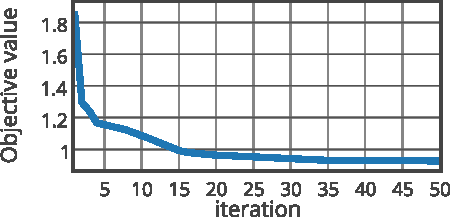
\includegraphics[height=0.25\linewidth]{./Multicontact/MulticontactJustin/fig/objective_function_walk.pdf}
		\caption{Experiment 1: Evolution of the cost function along the iterations.}
		\label{fig:objective_walk}
\end{figure}
The overall movement is depicted in Fig.~\ref{fig:moviepicture} (see also the accompanying video). The steps are very large for the humanoid robot (which is $1.60\,$m tall).

Fig. \ref{fig:zmp_walk} shows the ZMP trajectory on the Y axis resulting from the OCP, compared to the estimation coming from force sensors measurement. The ZMP is very similar to what could be obtained by a classical WPG with assumption of flat contact. The proper tracking on the real robot shows the dynamic consistency of the output of the OCP.

\begin{figure}[!ht]
	\centering
	\begin{tikzpicture}
    \node (fig) at (0,0) {
      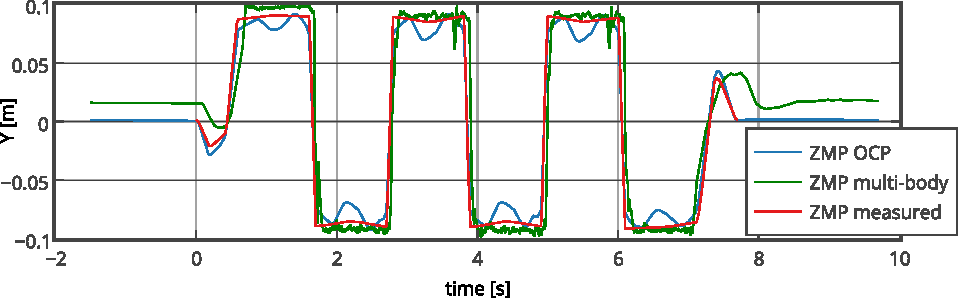
\includegraphics[height=0.25\linewidth]
      {/Multicontact/MulticontactJustin/fig/zmp-walk-45cm.pdf}
    };
% The arrows
  % forward
  \draw [-,color=red,        line width=0.3mm] (3.68,-0.04) -- node [] {} (4.33,-0.04);
  \draw [-,color=blue!40,    line width=0.3mm] (3.68,-0.44) -- node [] {} (4.33,-0.44);
  \draw [-,color=ForestGreen,line width=0.3mm] (3.68,-0.84) -- node [] {} (4.33,-0.84);
  \end{tikzpicture}
	\caption{Experiment 1: ZMP trajectories obtained from the OCP, the multi-body dynamics and the measurements.}
		\label{fig:zmp_walk}
\end{figure}

\begin{figure*}[!ht]
  \begin{center}
  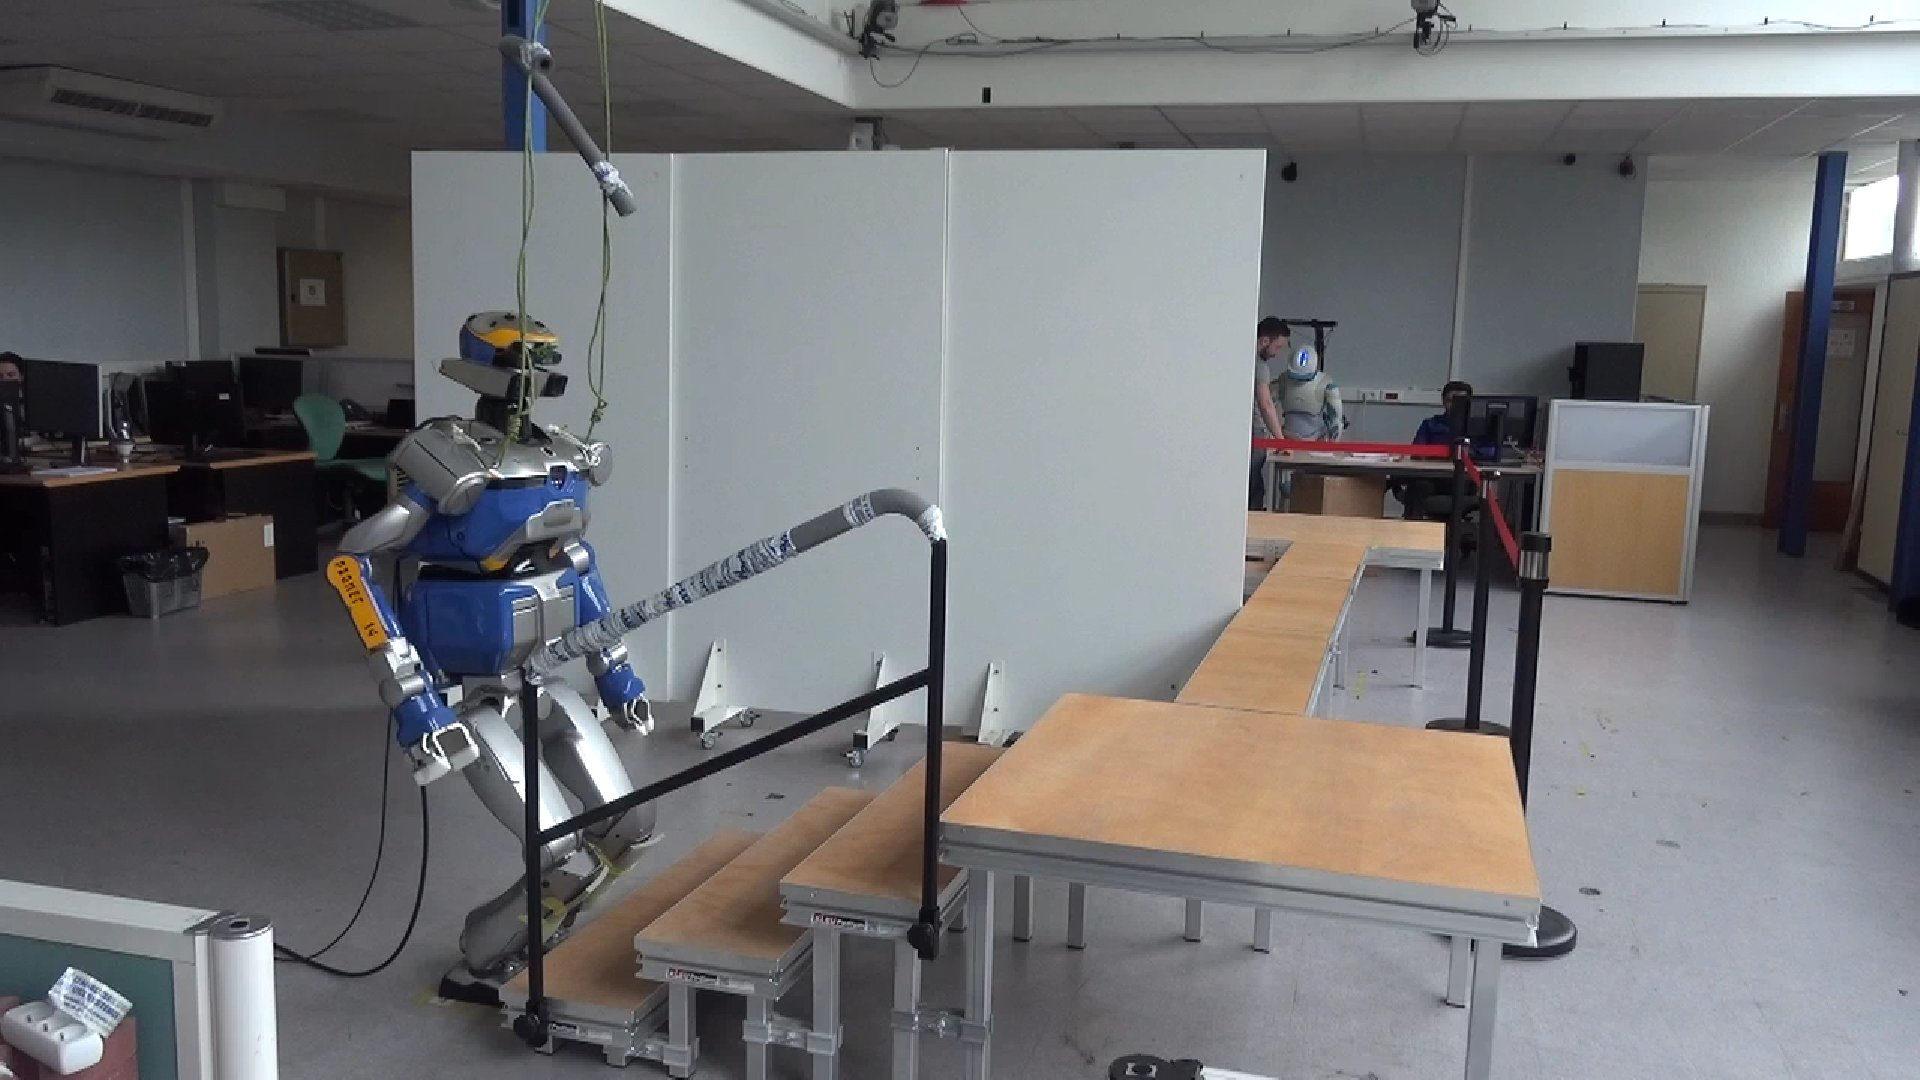
\includegraphics[trim={7.0cm 0.0cm 20.0cm 0.0cm}, clip, width=0.18\linewidth]
    {./Multicontact/MulticontactJustin/fig/stairclimbing1.jpeg}
  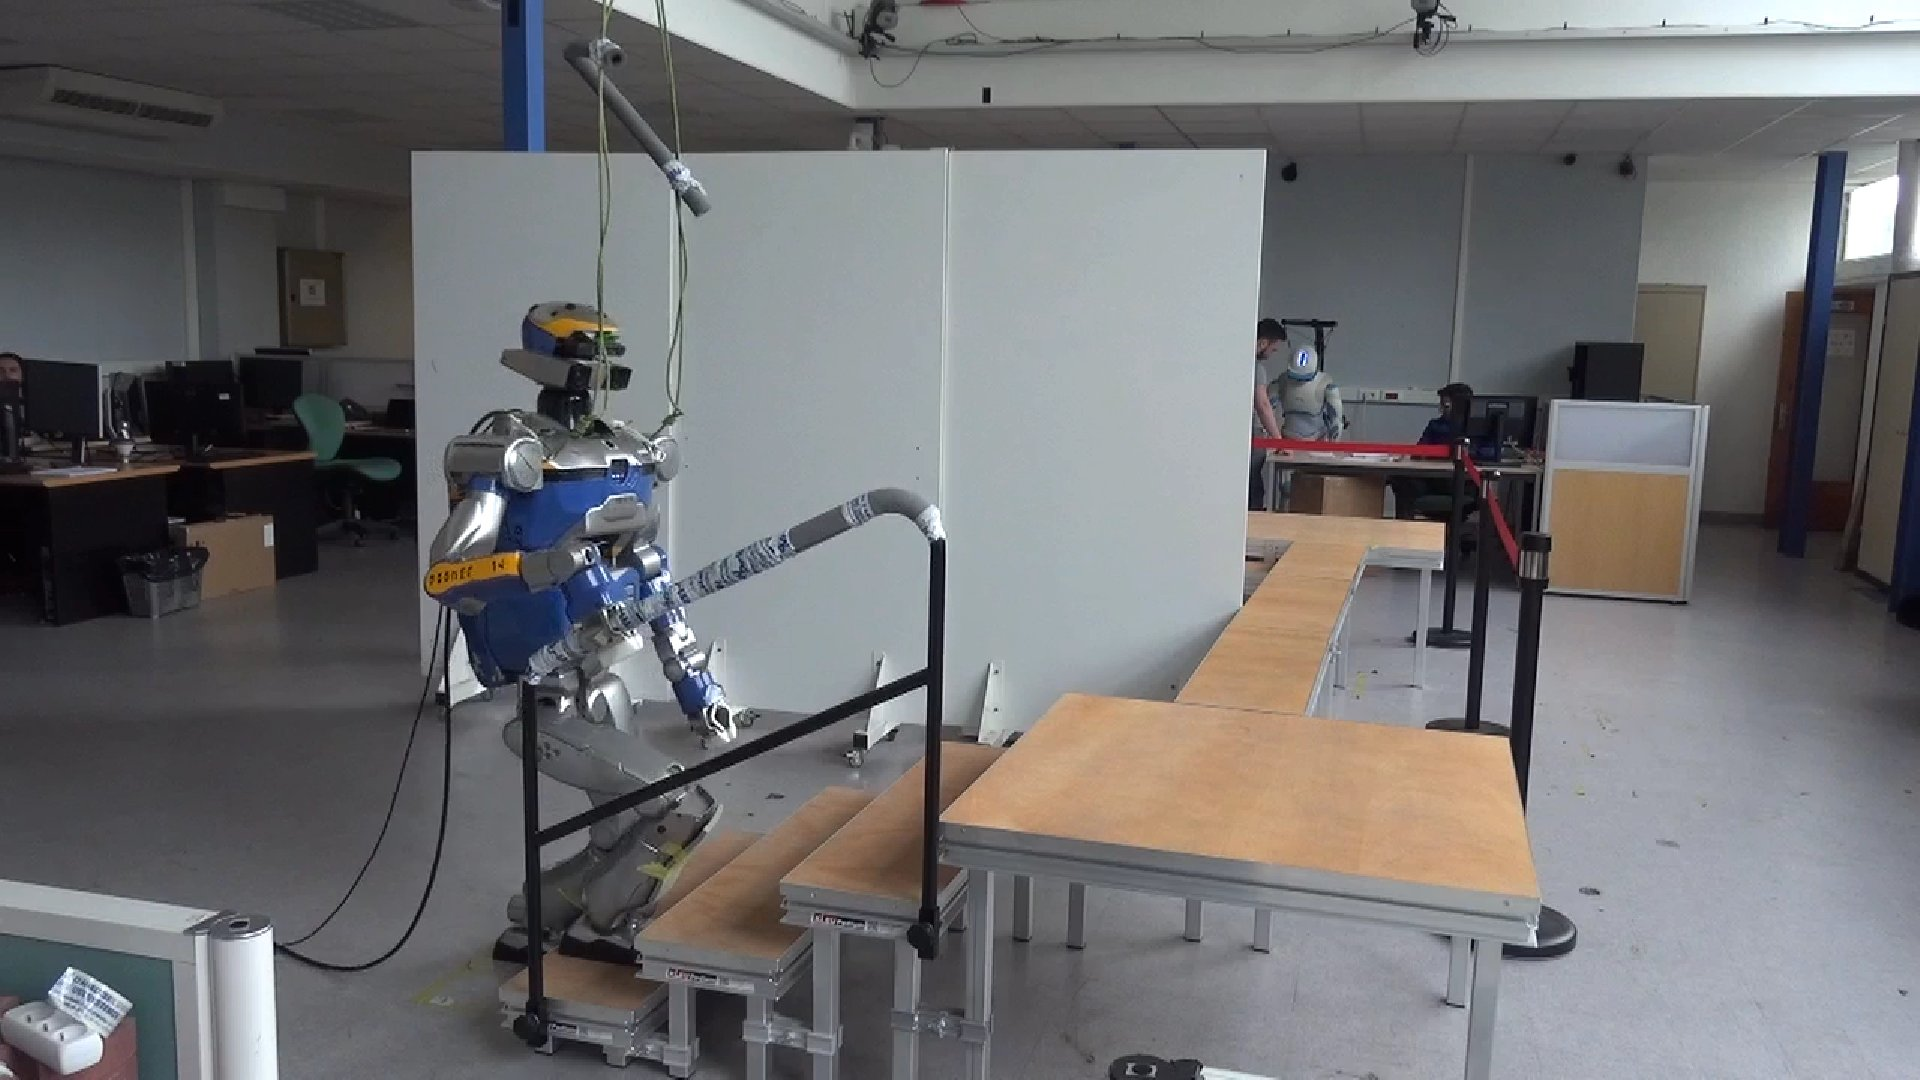
\includegraphics[trim={7.0cm 0.0cm 20.0cm 0.0cm}, clip, width=0.18\linewidth]
    {./Multicontact/MulticontactJustin/fig/stairclimbing2.jpeg}
  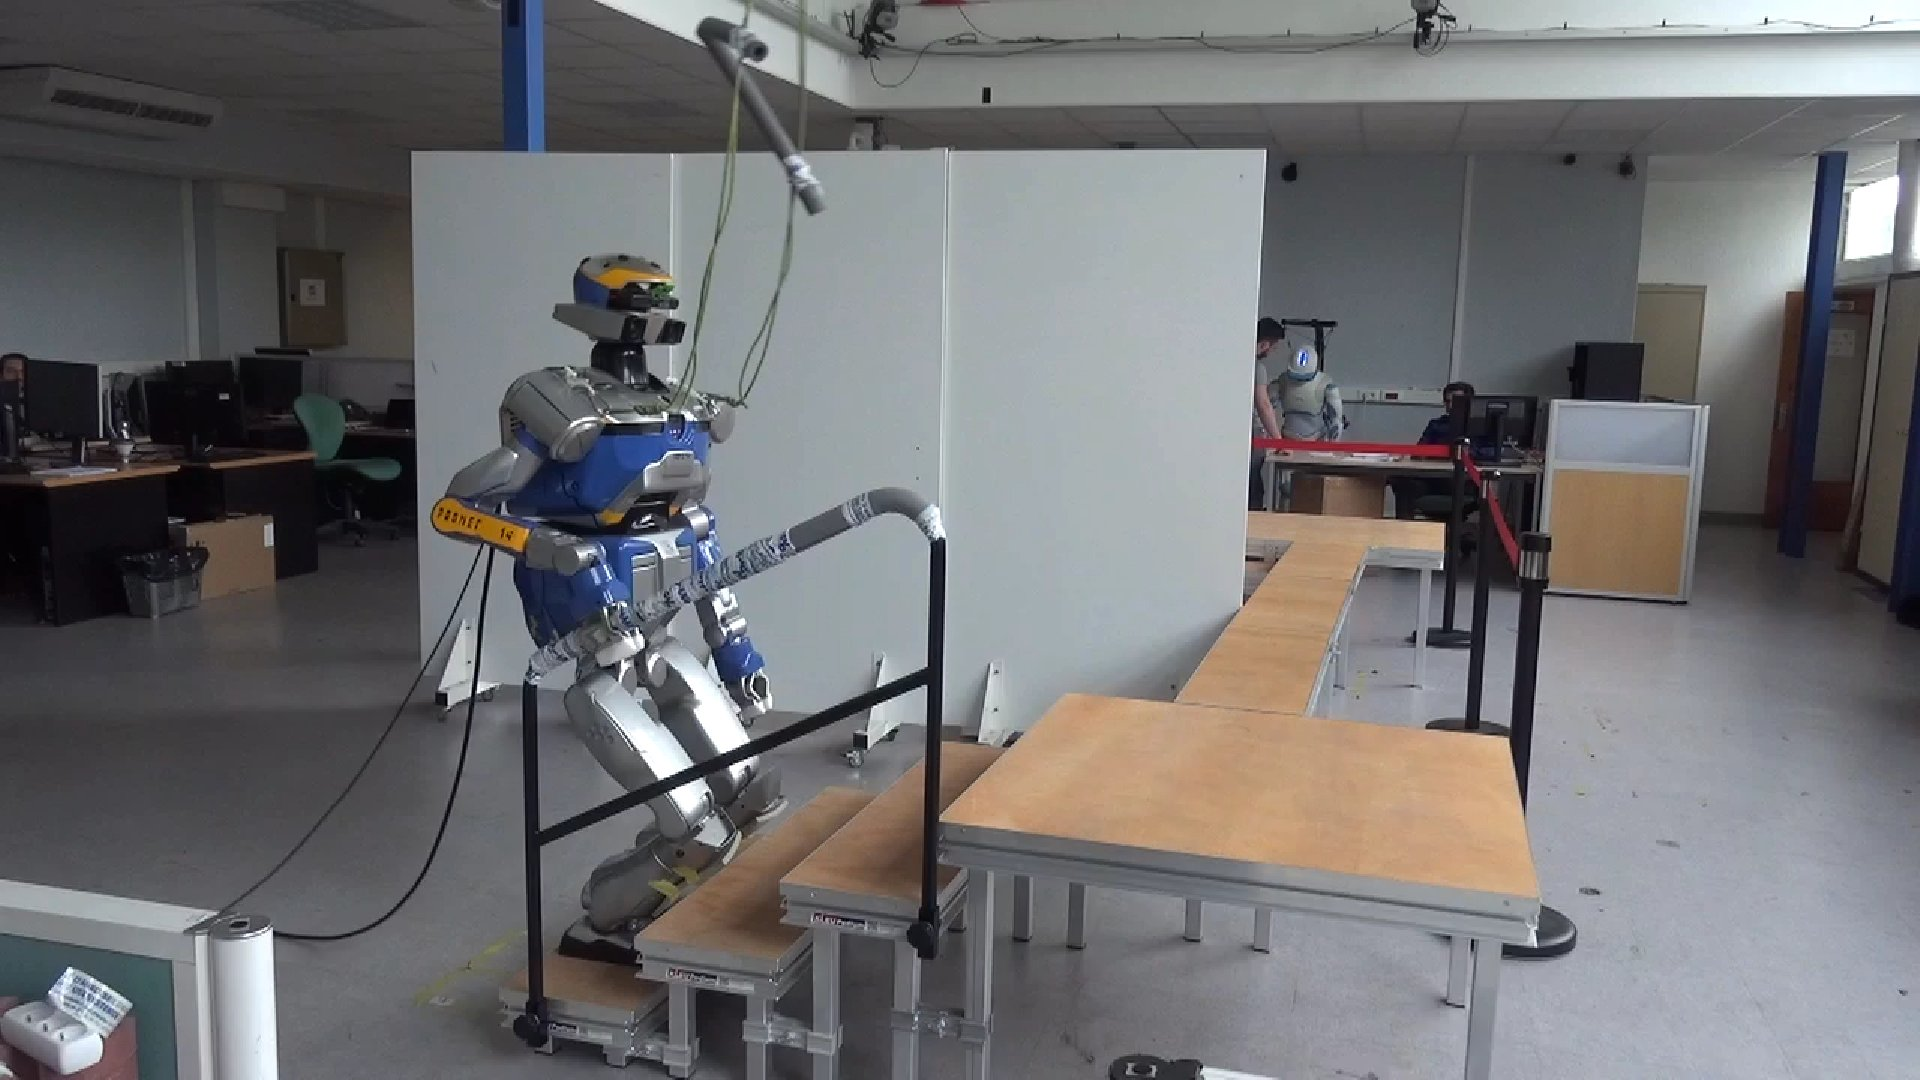
\includegraphics[trim={7.0cm 0.0cm 20.0cm 0.0cm}, clip, width=0.18\linewidth]
    {./Multicontact/MulticontactJustin/fig/stairclimbing3.jpeg}
  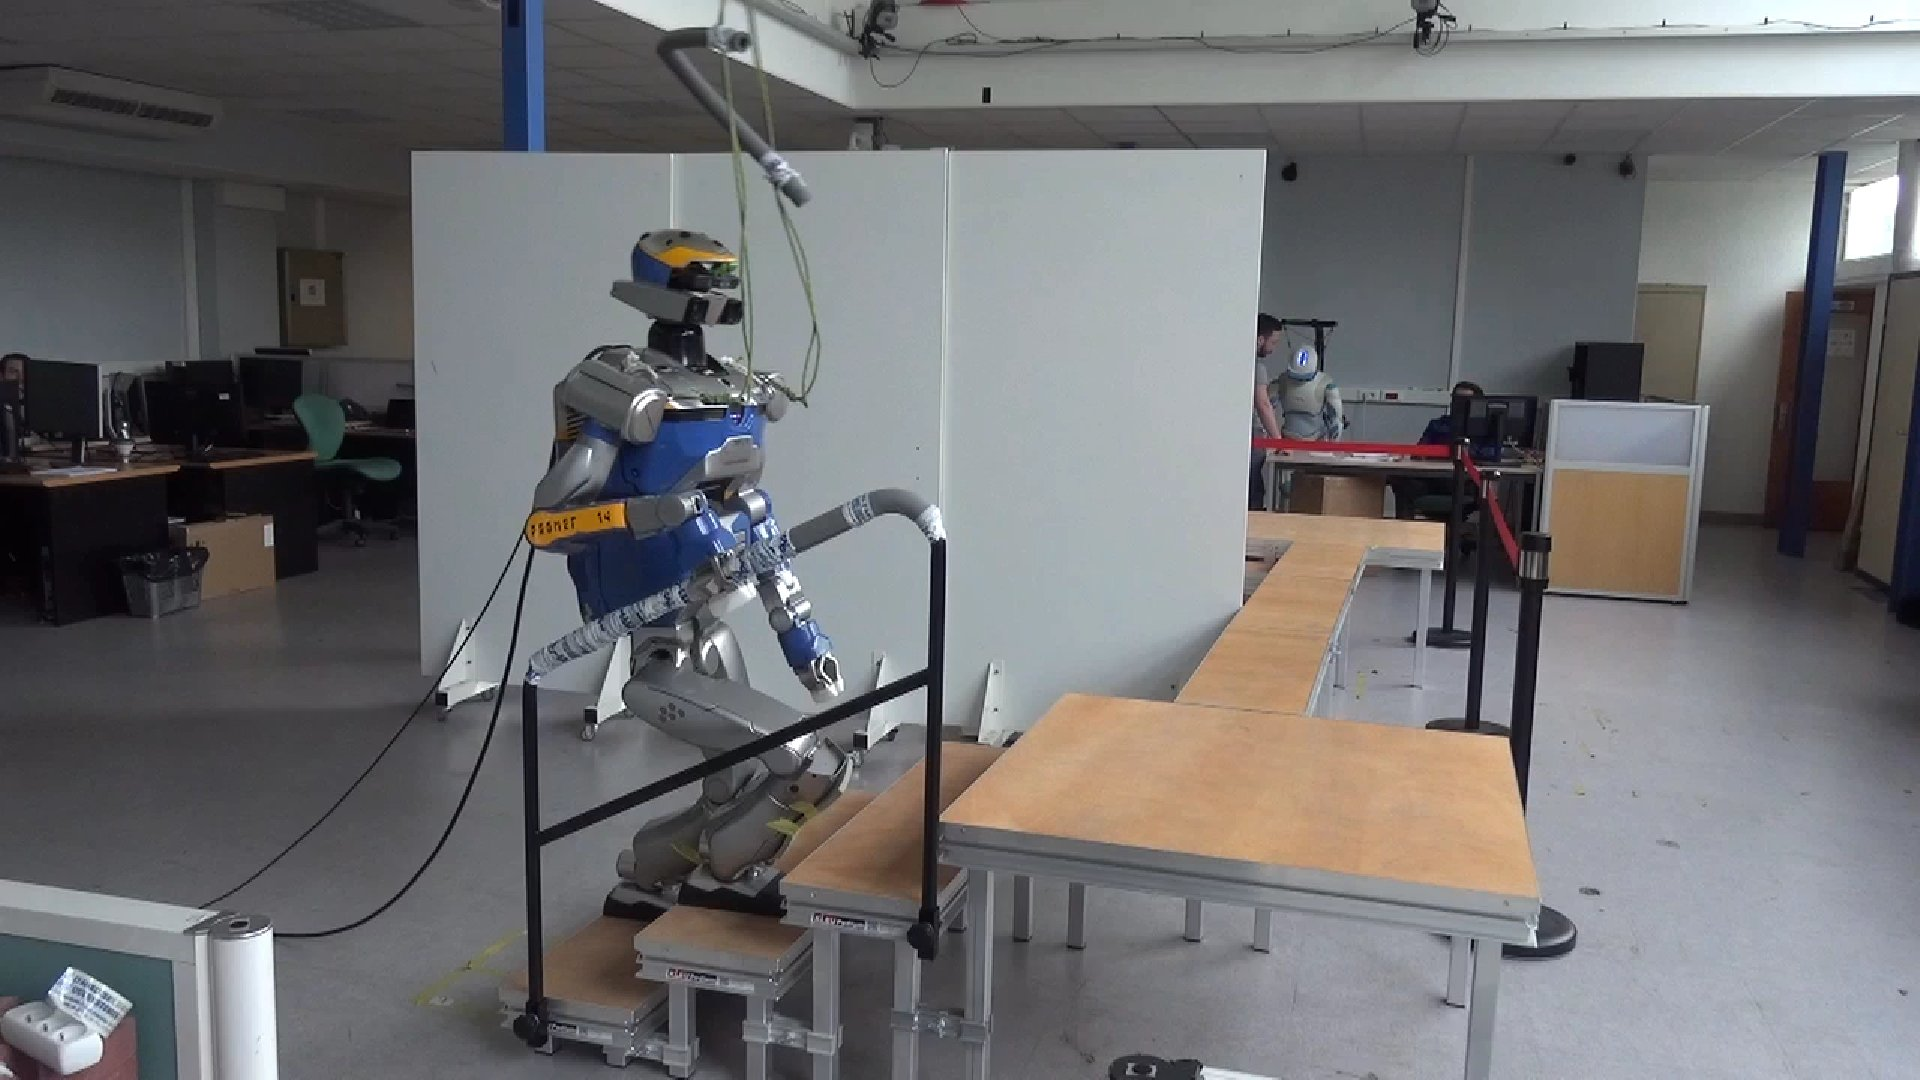
\includegraphics[trim={7.0cm 0.0cm 20.0cm 0.0cm}, clip, width=0.18\linewidth]
    {./Multicontact/MulticontactJustin/fig/stairclimbing4.jpeg}
  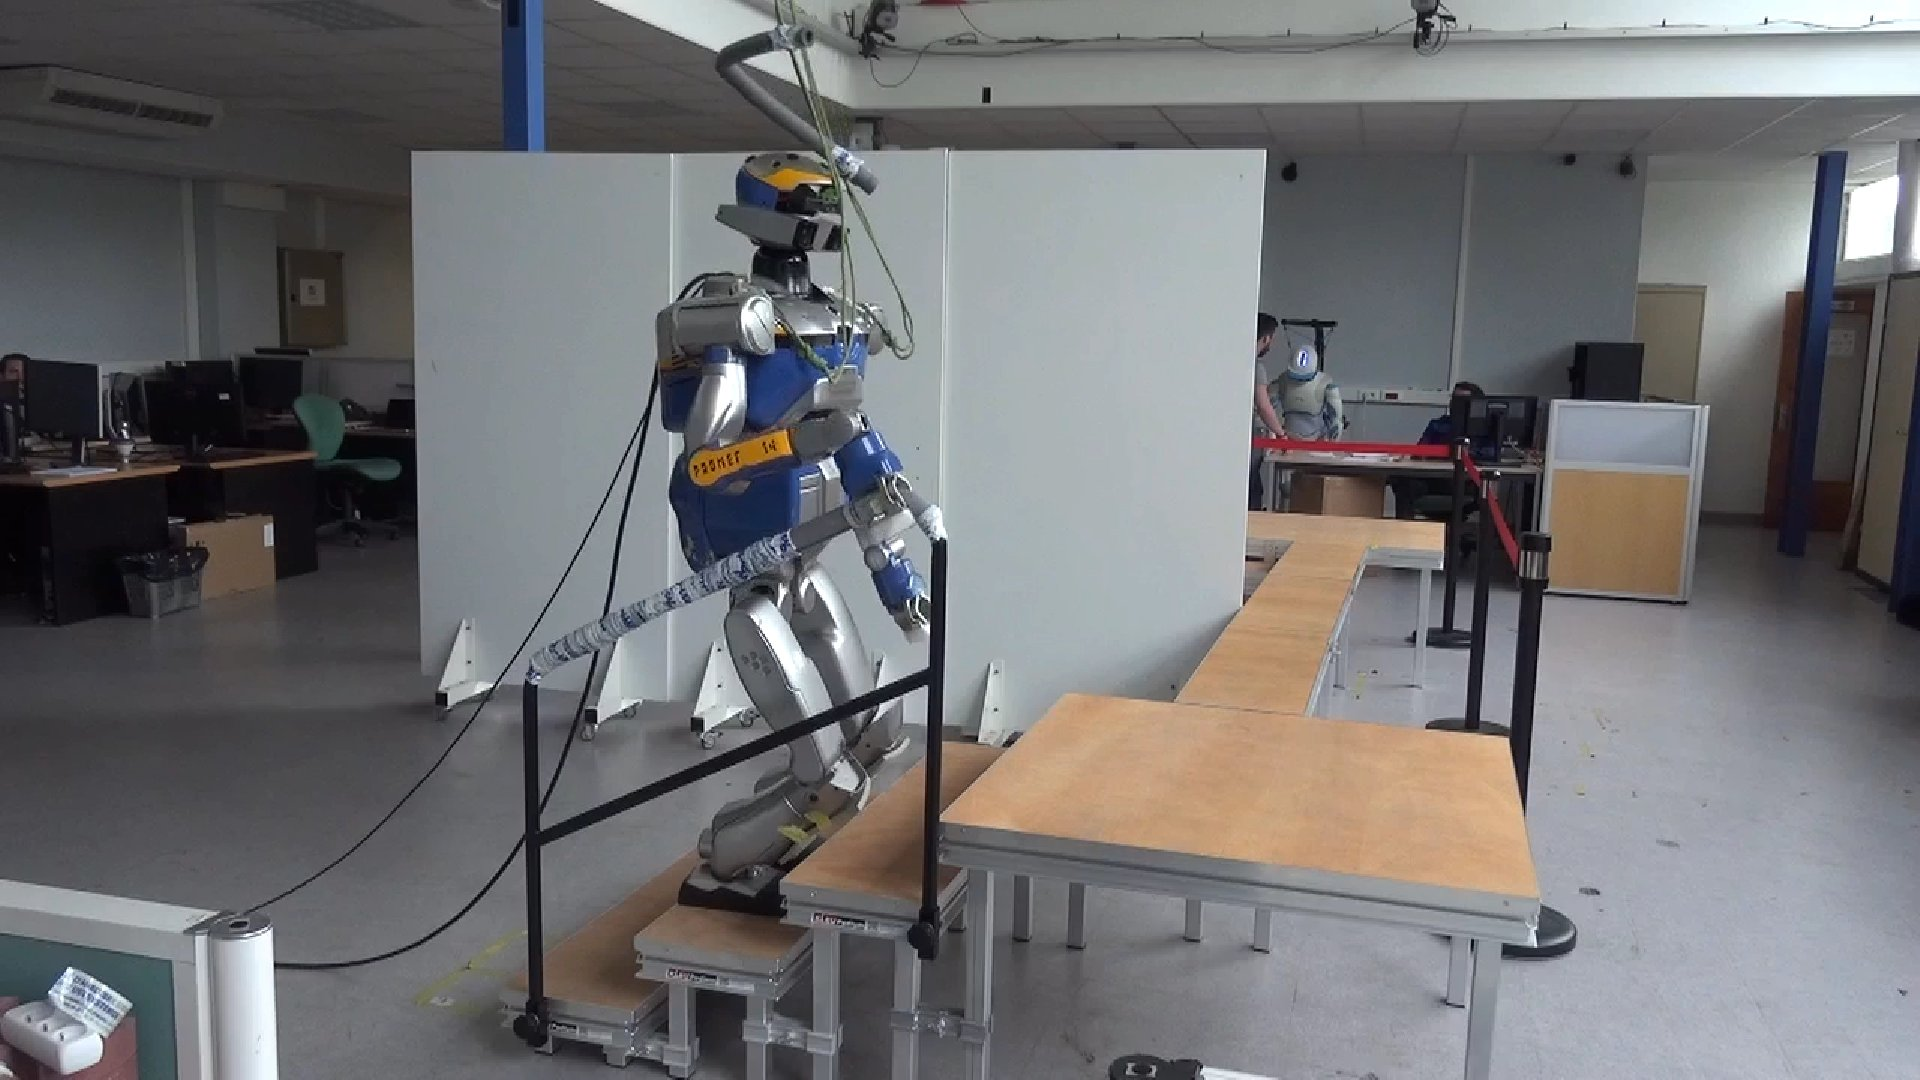
\includegraphics[trim={7.0cm 0.0cm 20.0cm 0.0cm}, clip, width=0.18\linewidth]
    {./Multicontact/MulticontactJustin/fig/stairclimbing5.jpeg}
  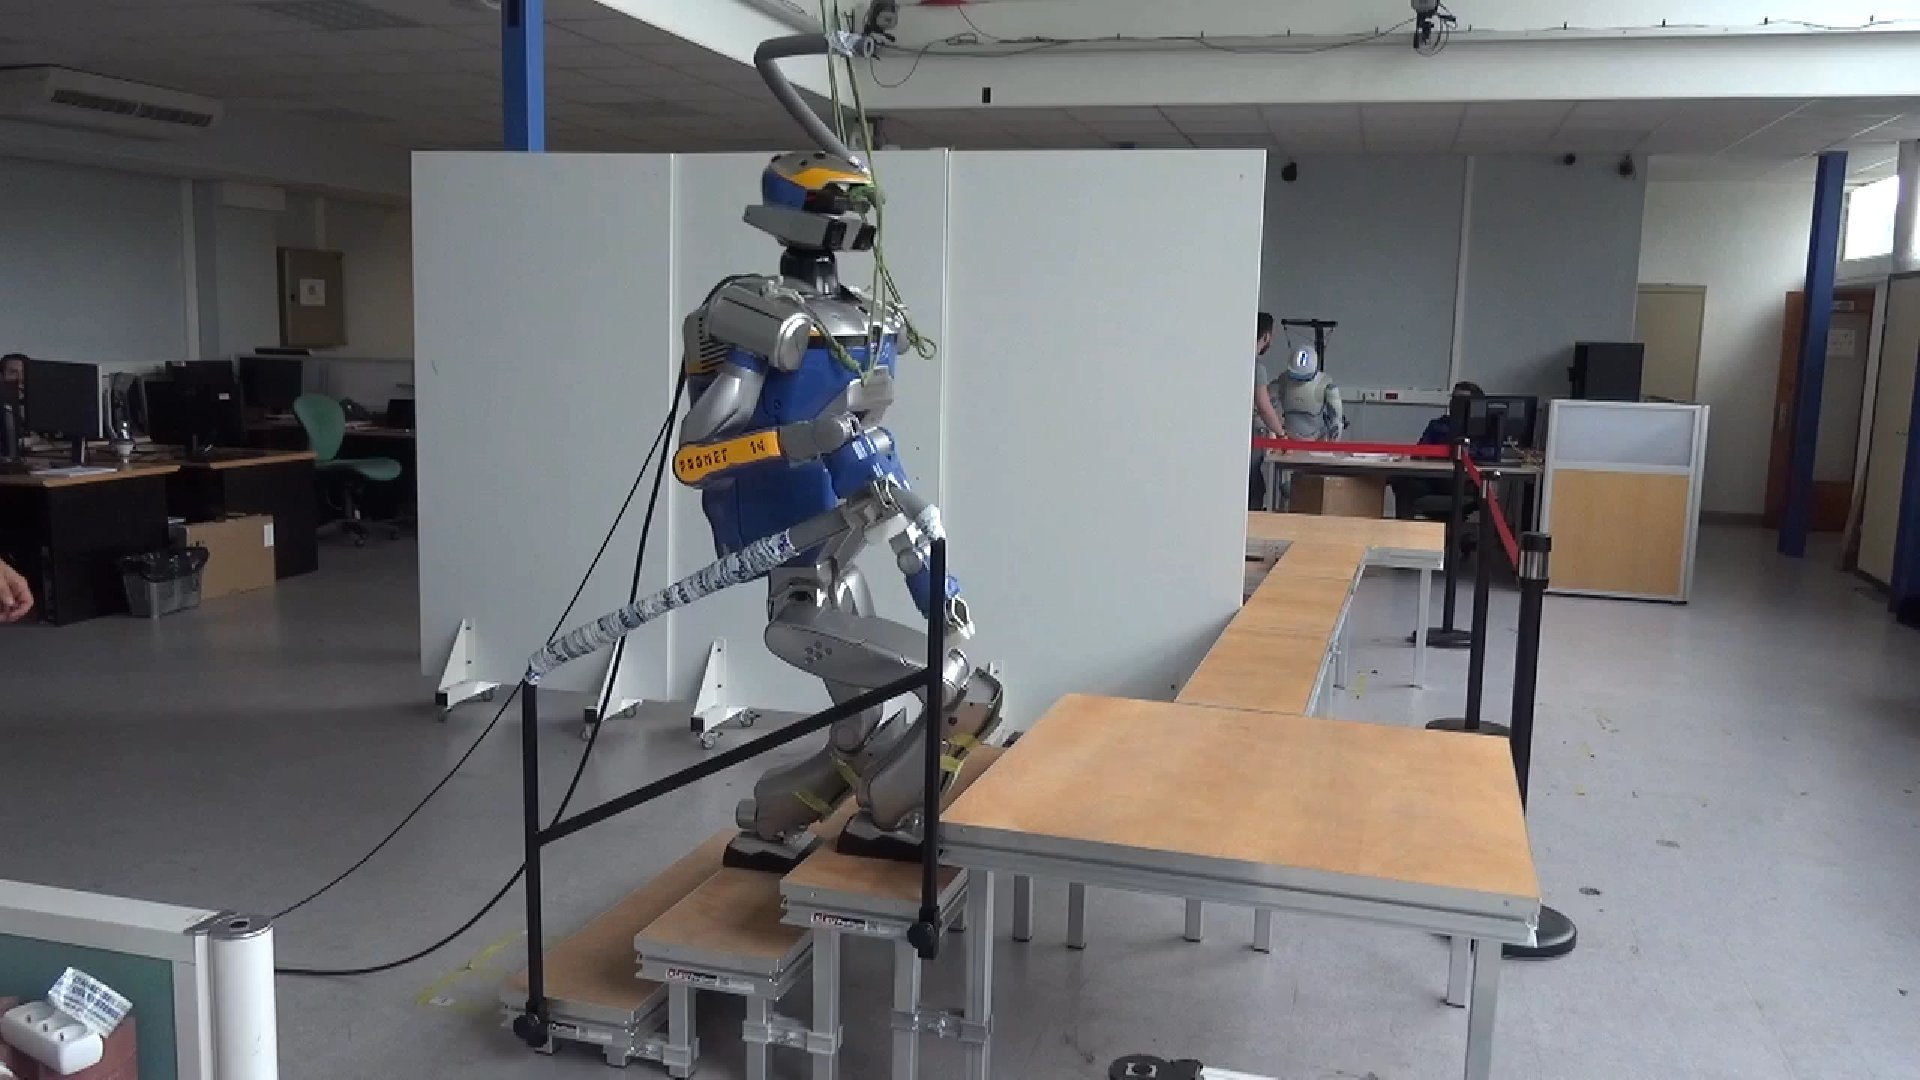
\includegraphics[trim={7.0cm 0.0cm 20.0cm 0.0cm}, clip, width=0.18\linewidth]
    {./Multicontact/MulticontactJustin/fig/stairclimbing6.jpeg}
  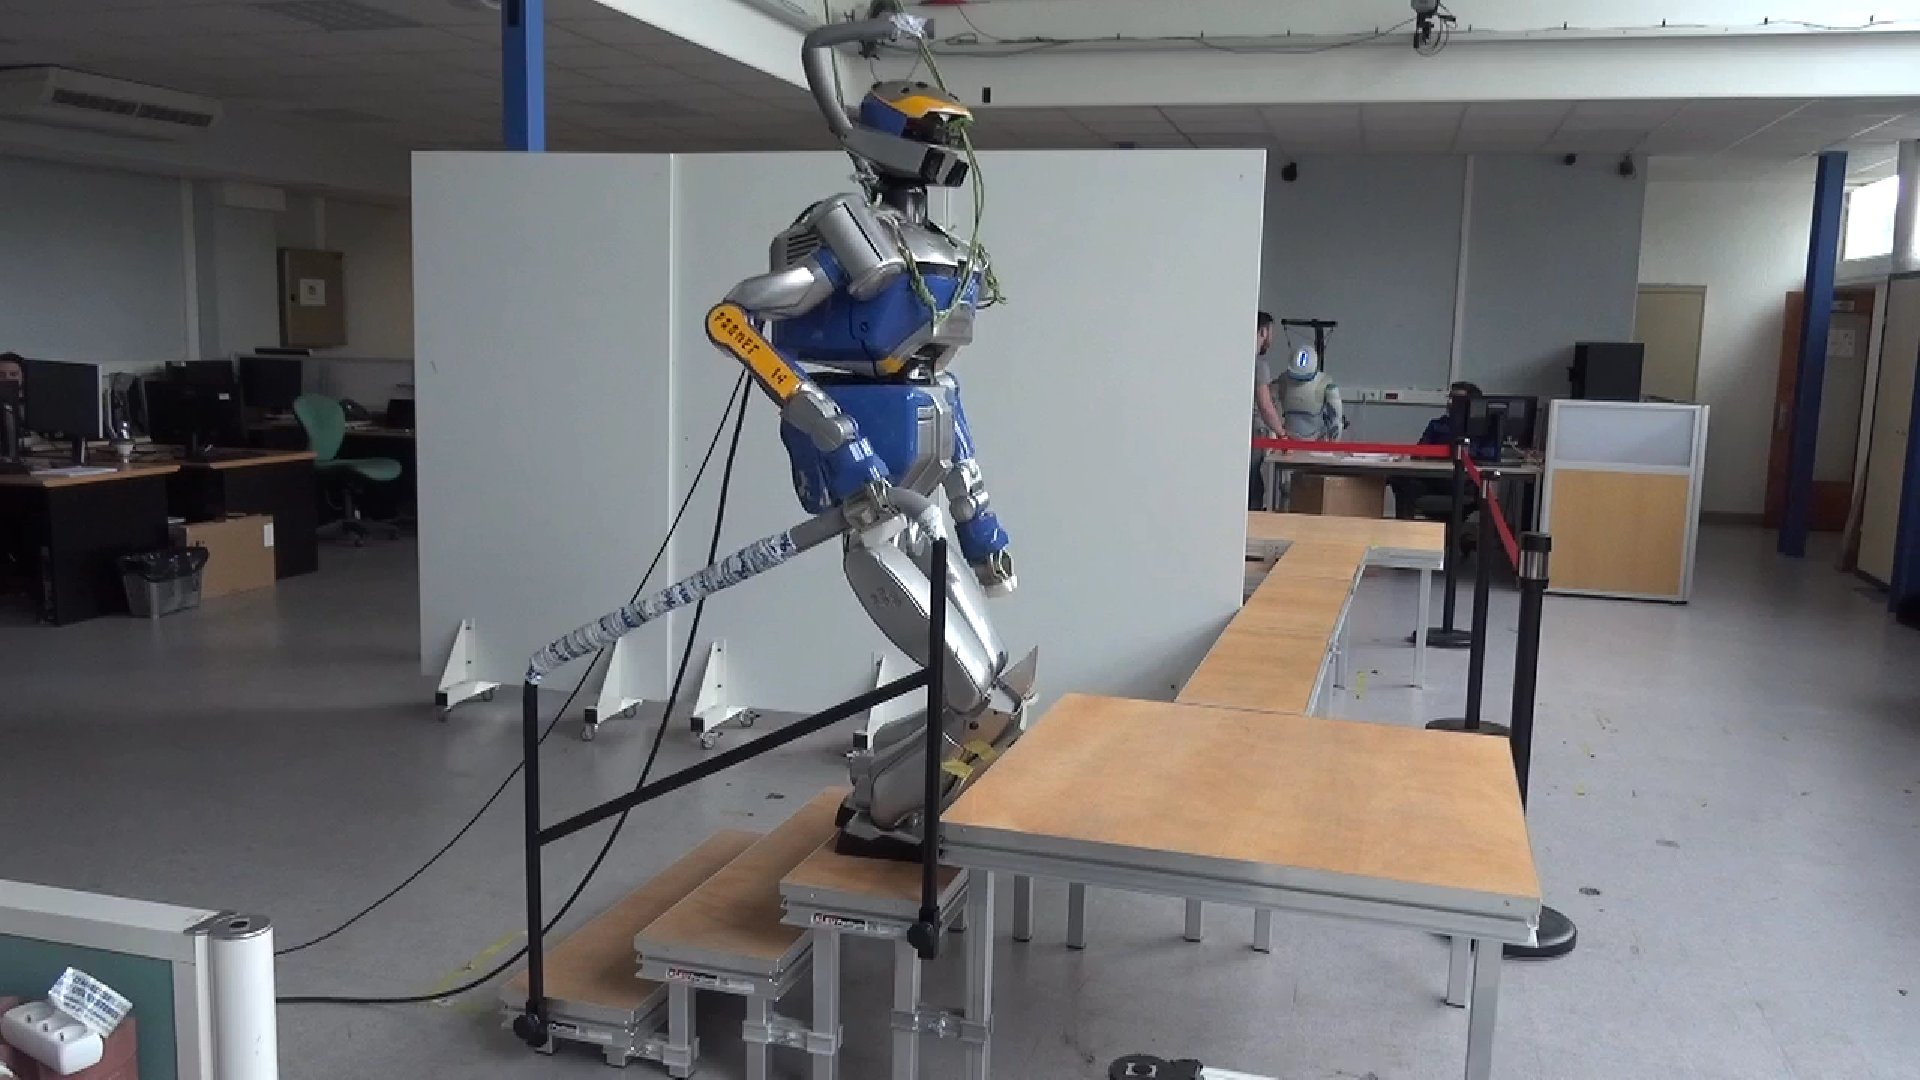
\includegraphics[trim={7.0cm 0.0cm 20.0cm 0.0cm}, clip, width=0.18\linewidth]
    {./Multicontact/MulticontactJustin/fig/stairclimbing7.jpeg}
    %trim={<left> <lower> <right> <upper>}
  \caption{
   Experiment 2: Climbing the stairs of $15cm$ height while using the handrail.
  }
  \label{fig:moviepicture2}
  \end{center}
\end{figure*}

\subsubsection*{Experiment 2: Climbing stairs equipped with a handrail}

In the climbing scenario, the contact sequence given by the planner is not cyclic anymore and takes around $1s$ to be computed. The computation of a feasible trajectory to climb one stair is done in less than $5.5s$ after $85$ iterations. 

Fig. \ref{fig:foot_forces} illustrates both the forces computed by the solver and the forces exerted on the real robot.
The simulated and measured forces do not match exactly but they have similar variations.
In both cases, we observe that the robot makes use of its right hand either for pulling or pushing.
The oscillations in the forces response are mainly due to the presence of a flexibility part in the robot's feet and to the compliance of the handrail.
These two physical disturbances are not considered in our framework.

\begin{figure}[!ht]
	\centering
	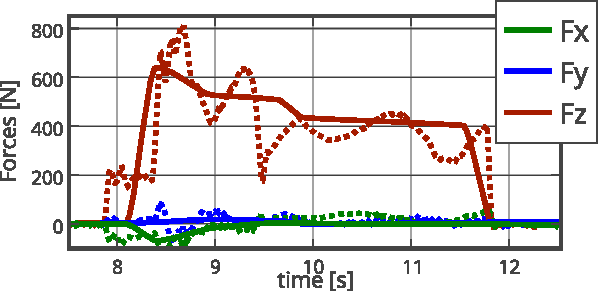
\includegraphics[width=0.4\linewidth]{./Multicontact/MulticontactJustin/fig/Right_Foot_Forces.pdf}
	\hspace*{1cm}
	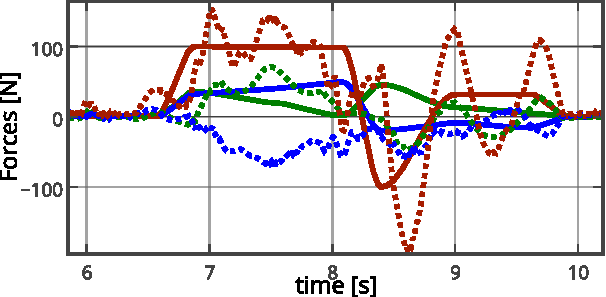
\includegraphics[width=0.4\linewidth]{./Multicontact/MulticontactJustin/fig/Right_Hand_Forces.pdf}
		\caption{Experiment 2: Reference (solid line) and measured (doted line) forces at the right foot (on the left) and hand (on the right) during one contact phase. The reference forces are properly tracked (even if some flexibility can be observed).}
		\label{fig:foot_forces}
\end{figure}
